\section{Direct Clustering and Density Estimation} 

  \subsection{K Means Clustering} 

    The simplest type of unsupervised learning is \textbf{clustering}. In the clustering problem, we are given a training set of \textit{unlabeled} data

    \begin{equation}
      \{ \mathbf{x}^{(1)}, \mathbf{x}^{(2)}, \ldots, \mathbf{x}^{(n)}\}
    \end{equation}
    and want to group the data into a few cohesive ``clusters.''

    \begin{enumerate}
      \item Determine the number of clusters that we want to find and set it as $k$ (this can be a disadvantage if we do not know how many clusters we are looking for beforehand).

      \item We initialize the \textbf{cluster centroids} $\boldsymbol{\mu}_1, \boldsymbol{\mu}_2, \ldots, \boldsymbol{\mu}_k \in \mathbb{R}^d$ randomly or by some other method.

      \item The next part takes the centroids and moves them to the center of each cluster accordingly. The following two steps are repeated until convergence (and convergence is guaranteed):
        \begin{enumerate}
          \item We assign each training sample $\mathbf{x}^{(i)}$ to the closest cluster centroid $\boldsymbol{\mu}_j$. That is, for every $i = 1, \ldots, n$, set
            \begin{equation}
              c^{(i)} \equiv \text{arg}\; \min_j || \mathbf{x}^{(i)} - \boldsymbol{\mu}_j ||^2
            \end{equation}
          where this $\text{argmin}$ function returns the input to a function that yields the minimum (in this case, the number $j$ that yields the minimum value of $|| \mathbf{x}^{(i)} - \boldsymbol{\mu}_j ||^2$ for each $i$).

          \item We move each training cluster centroid $\boldsymbol{\mu}_j$ to the mean of the points assigned to it. That is, for each $j = 1, \ldots, k$, set 
            \begin{equation}
              \boldsymbol{\mu}_j \equiv \frac{\sum_{i=1}^n 1\{c^{(i)} = j\}\, \mathbf{x}^{(i)}}{\sum_{i=1}^n 1 \{c^{(i)} = j\}}
            \end{equation}
        \end{enumerate}
    \end{enumerate}

    \begin{figure}[H]
      \centering 
      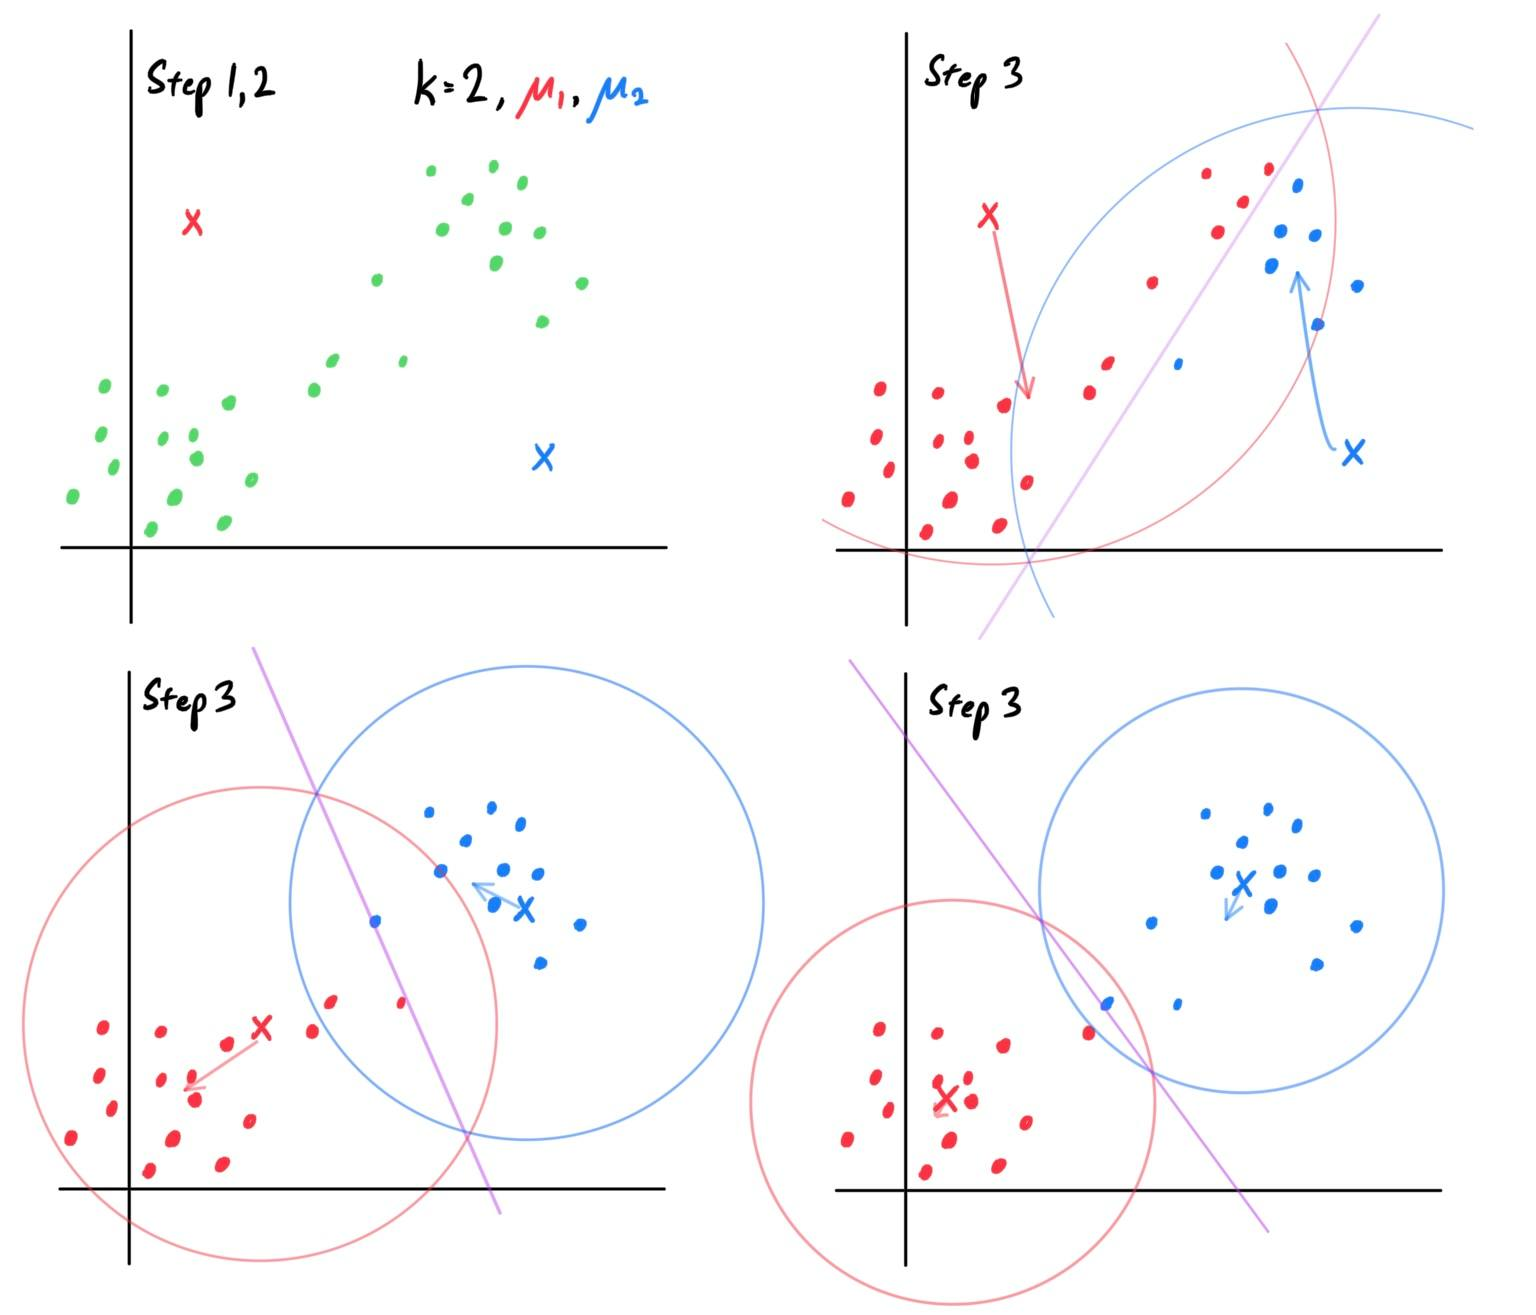
\includegraphics[scale=0.25]{img/k_means_clustering.jpg}
      \caption{The steps can be visualized for a set of unlabeled data (green points) in $\mathbb{R}^2$ clustered into $k=2$ groups (red and blue). The crosses represent the cluster centroids.} 
      \label{fig:k_means_clustering}
    \end{figure}

    We can interpret this algorithm in another equivalent way. $k$-means is precisely coordinate descent on the cost function called the \textbf{distortion function}: 
    \begin{equation}
      L(\boldsymbol{\mu}_1, \ldots, \boldsymbol{\mu}_k) \equiv \sum_{i=1}^n \min_k ||\mathbf{x}^{(i)} - \boldsymbol{\mu}_k ||^2
    \end{equation}
    but since $L$ is not necessarily convex, it might be susceptible to local extrema.

  \subsection{Kernel Density Estimation}

